\documentclass[11pt,a4paper]{article}
\usepackage[utf8]{inputenc}
\usepackage[spanish]{babel}
\usepackage[margin=17mm]{geometry}
\usepackage{amsmath,amssymb}
\usepackage{graphicx}
\usepackage{xcolor}
\usepackage{hyperref}
\usepackage{booktabs}
\usepackage{tabularx}
\usepackage{titlesec}
\usepackage{tcolorbox}
\usepackage{enumitem}
\usepackage{fancyhdr}

% Definición de Paleta de Colores
\definecolor{mainblue}{RGB}{24, 119, 242}
\definecolor{darkbg}{RGB}{18, 18, 18}
\definecolor{headerblue}{RGB}{33, 150, 243}
\definecolor{numred}{RGB}{211, 47, 47}
\definecolor{lightgray}{RGB}{240, 242, 245}

% Estilo de Encabezados y Pies de Página
\pagestyle{fancy}
\fancyhf{}
\lhead{\small\textbf{FTIRdex} --- Manual de Usuario}
\rhead{\small Versión 0.0.5}
\cfoot{\thepage}

\hypersetup{
    colorlinks=true,
    linkcolor=mainblue,
    urlcolor=mainblue,
    pdftitle={FTIRdex - Manual de Usuario},
    pdfauthor={FTIRdex Dev Team}
}

% Personalización de Secciones
\titleformat{\section}{\Large\bfseries\color{mainblue}}{\thesection}{1em}{}
\titleformat{\subsection}{\large\bfseries\color{darkgray}}{\thesubsection}{1em}{}

\begin{document}

% --- CARÁTULA ---
\begin{titlepage}
    \centering
    \vspace*{0.8cm}
    
    % Icono oficial ampliado (4.8 cm)
    
\includegraphics[width=4.8cm]{../../assets/icono.png}\\[0.6cm]
    
    {\Huge\bfseries\color{mainblue} FTIRdex}\\[0.3cm]
    {\huge Software de Análisis y Procesamiento\\de Espectroscopia FTIR}\\[1.2cm]
    
    \begin{tcolorbox}[colback=lightgray,colframe=mainblue,arc=4mm,width=0.88\linewidth,halign=center]
        {\Large\bfseries Manual de Usuario y Guía de Operación}\\[0.2cm]
        {\small Documentación Oficial del Sistema}
    \end{tcolorbox}
    
    \vfill
    
    \begin{minipage}{0.45\textwidth}
        \begin{flushleft} \large
            \textbf{Propiedad Intelectual:}\\
            Ing. Mendoza Pablo Nicolás\\
            \small\textbf{UTN FRLP}
        \end{flushleft}
    \end{minipage}
    \begin{minipage}{0.45\textwidth}
        \begin{flushright} \large
            \textbf{Desarrollador (DEV):}\\
            Alemán Matías Roberto\\
            \small\textbf{UTN FRLP}
        \end{flushright}
    \end{minipage}
    
    \vspace{1.5cm}
    {\large Julio 2026 --- Versión 0.0.5}
\end{titlepage}

\tableofcontents
\newpage

% --- 1. INTRODUCCIÓN ---
\section{Introducción y Arquitectura del Sistema}
\textbf{FTIRdex} es una aplicación de escritorio nativa y liviana diseñada para la importación, preprocesamiento numérico, detección de picos y visualización interactiva de espectros de espectroscopia de infrarrojo por transformada de Fourier (FTIR).

El proyecto se encuentra seccionado internamente en tres tecnologías principales:

\begin{enumerate}[leftmargin=*,label=\textbf{\arabic*.}]
    \item \textbf{Interfaz Gráfica (GUI) ultra-fluida:} Desarrollada nativamente en C (\texttt{libnativegui}).
    \item \textbf{Motor de Procesamiento Científico:} Desarrollado en Python (\texttt{FTIRlib}).
    \item \textbf{Sistema de Archivos Virtual (VFS):} Módulo para virtualizar y manipular los archivos de proyecto \texttt{.ftirzip} directamente como directorios en memoria (\texttt{libzipvfs}).
\end{enumerate}

\begin{tcolorbox}[colback=yellow!5!white,colframe=orange!80!black,title=\textbf{Aclaración sobre el Formato de Proyecto (.ftirzip)}]
El formato de archivo \texttt{.ftirzip} es técnicamente un contenedor estandarizado en formato \textbf{ZIP}. Por esta razón, el usuario puede cambiar la extensión a \texttt{.zip} o abrir el archivo directamente con cualquier gestor de archivos comprimidos (ej. WinRAR, 7-Zip, Explorador de Windows) para acceder manualmente a las imágenes y reportes de datos numéricos en su interior.
\end{tcolorbox}

\begin{tcolorbox}[colback=blue!5!white,colframe=mainblue,title=\textbf{Modalidades de Distribución}]
\begin{itemize}[leftmargin=*]
    \item \textbf{Instalador ejecutable (\texttt{FTIRdex-0.0.5-installer-x64.exe}):} Instalación formal en Windows con registro de extensiones y desinstalador limpio libre de residuos de caché.
    \item \textbf{Versión Portable (\texttt{FTIRdex-0.0.5-portable.zip}):} Edición autocontenida que no requiere instalación previa ni permisos de administrador.
\end{itemize}
\end{tcolorbox}

% --- 2. ESTRUCTURA DE LA INTERFAZ ---
\section{Estructura de la Interfaz Principal}

Para facilitar la comprensión del entorno de trabajo, la interfaz de FTIRdex se organiza en \textbf{dos niveles de abstracción}: una visión macro de 4 grandes entidades y un desglose detallado de sus sub-herramientas.

\subsection{Primer Vistazo: Las 4 Entidades Gráficas Principales}
A nivel estructural macro, la pantalla se compone de cuatro zonas principales:

\begin{figure}[h!]
    \centering
    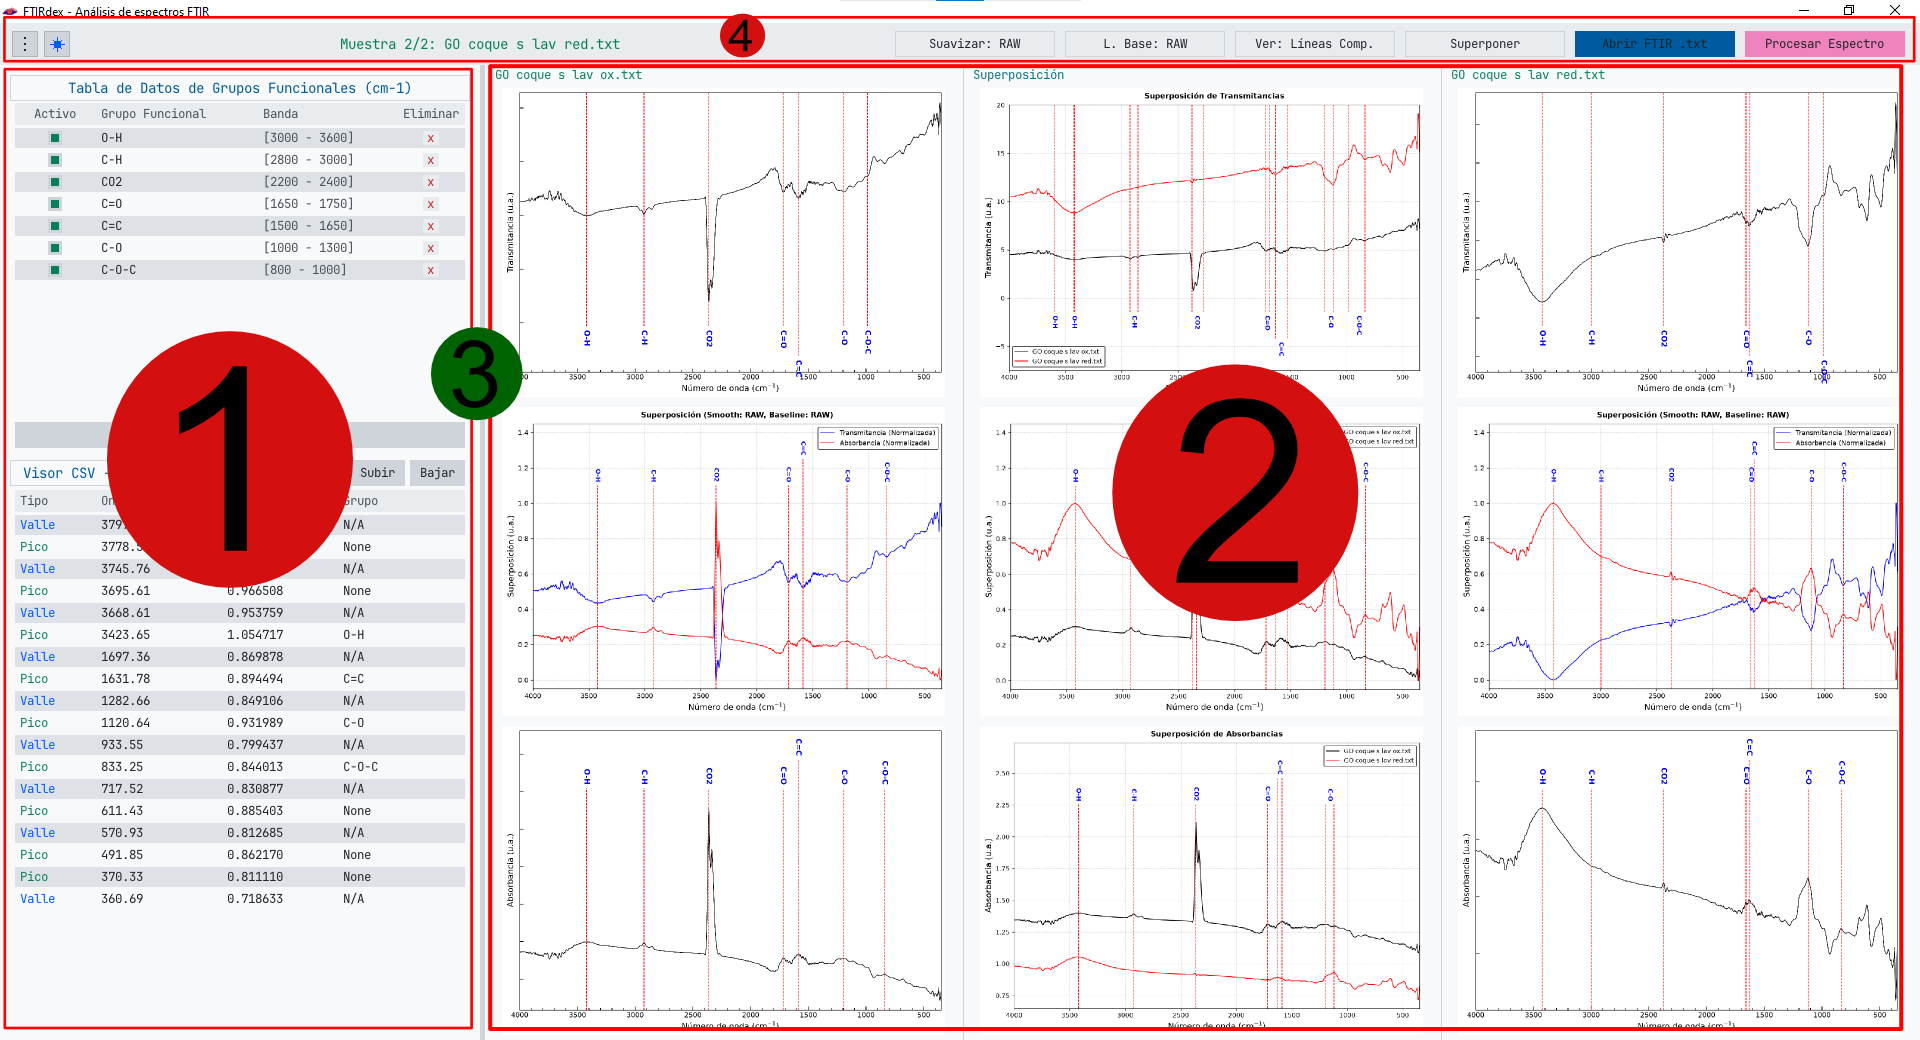
\includegraphics[width=0.96\linewidth]{../../assets/manual-main-interfaces.png}
    \caption{Esquema macro de las 4 grandes entidades estructurales de FTIRdex.}
    \label{fig:macro_interfaces}
\end{figure}

\begin{enumerate}[label=\textbf{\arabic*.}]
    \item \textbf{Panel Lateral Izquierdo (Control de Datos Numéricos):} Contenedor de las tablas de configuración de grupos funcionales y el visor tabular CSV de resultados.
    
    \item \textbf{Panel de Galería de Gráficos (Matriz de Espectros Adaptativa):} Espacio dedicado a la renderización visual de las curvas de espectroscopia, con un diseño adaptativo de 3 Filas $\times$ $N$ Columnas, donde respectivamente:
    \begin{itemize}[leftmargin=*]
        \item \textbf{Filas Horizontales (3):} Transmitancia, Superposición y Absorbancia.
        \item \textbf{Columnas Dinámicas ($N$):} Corresponden a cada muestra cargada, más la columna de superposición grupal comparativa.
    \end{itemize}
    
    \item \textbf{Barra Splitter Vertical:} Divisor de redimensionamiento dinámico que ajusta el ancho proporcional entre el panel izquierdo (1) y el panel de gráficos (2).
    
    \item \textbf{Barra de Herramientas Superior:} Franja superior que alberga las opciones globales de navegación, apertura de archivos y menús desplegables de procesamiento.
\end{enumerate}

\newpage
\subsection{Desglose Detallado de Sub-Herramientas (Referencias 1 al 7)}

En el mapa numérico detallado de la aplicación se identifican los siguientes elementos:

\begin{figure}[h!]
    \centering
    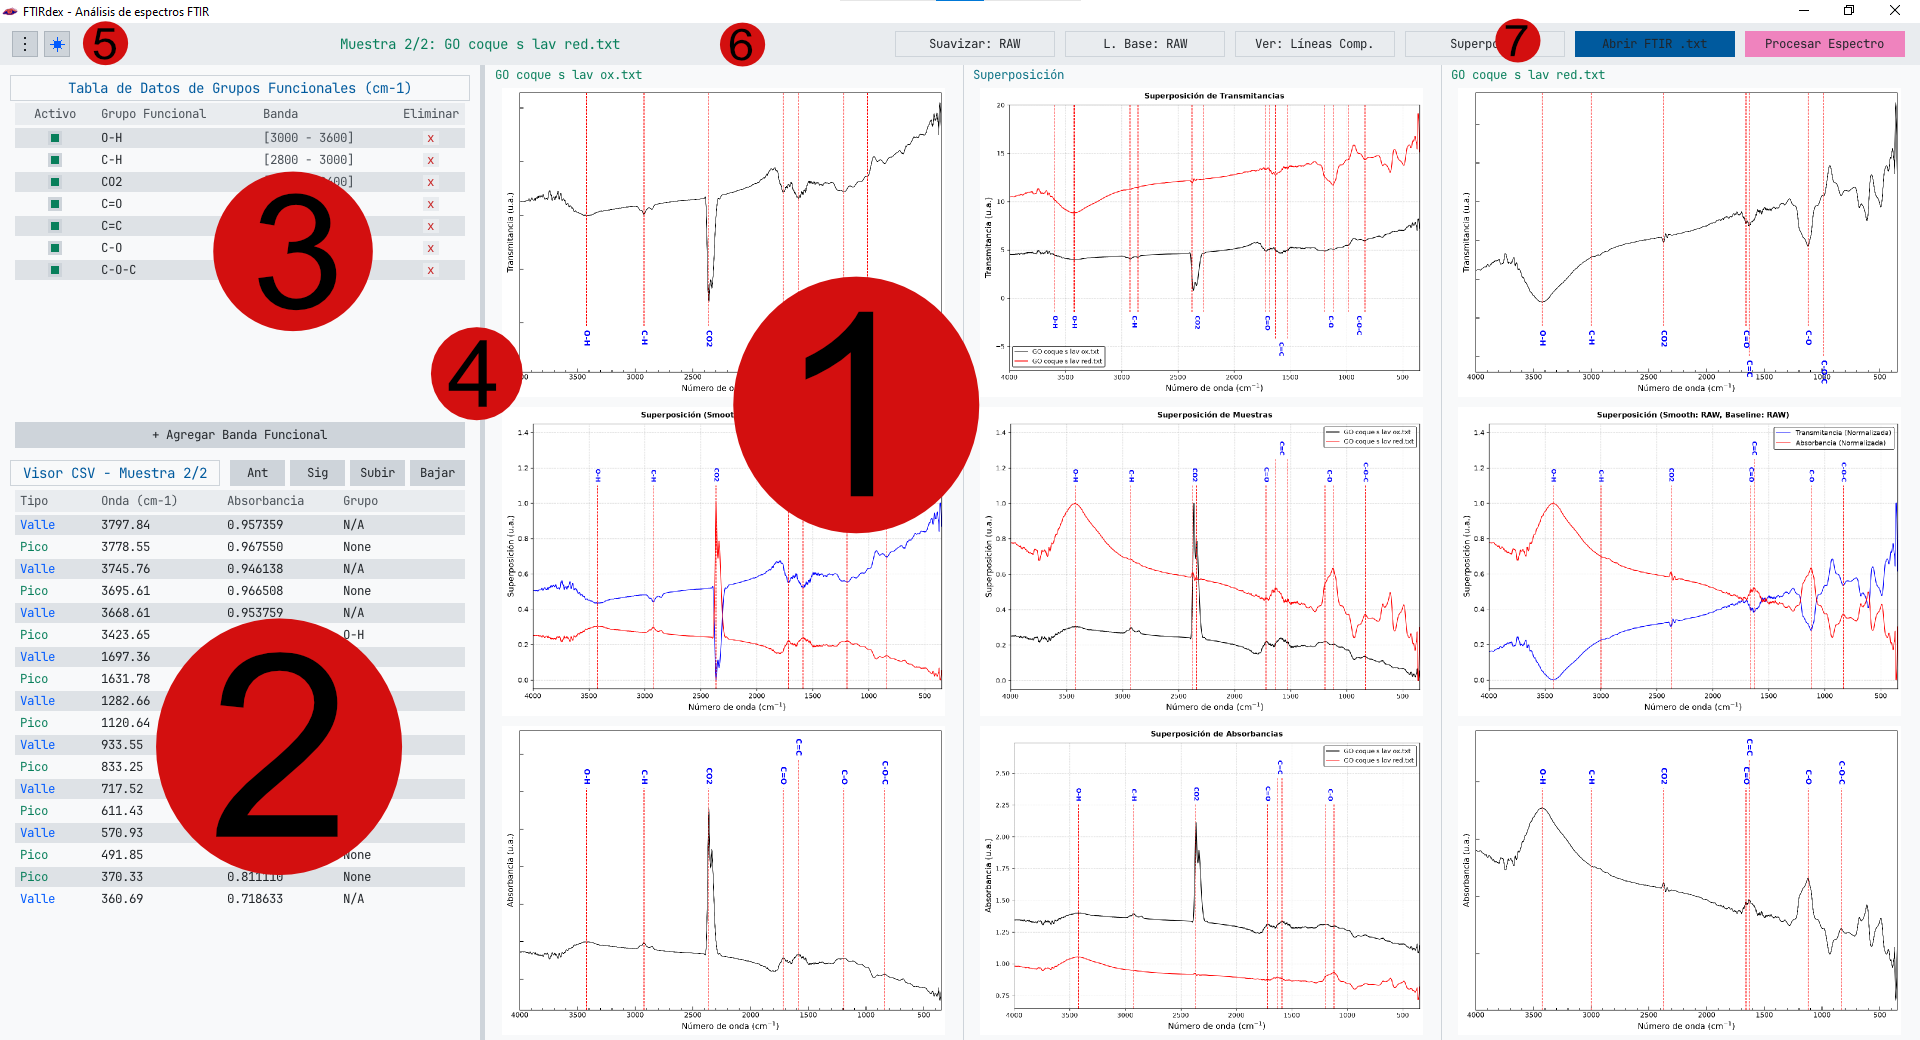
\includegraphics[width=0.96\linewidth]{../../assets/manual-interfaces-list.png}
    \caption{Mapa numérico detallado de sub-herramientas (Referencias 1 al 7).}
    \label{fig:interfaces_list}
\end{figure}

\begin{description}[font=\bfseries\color{numred}]
    \item[{[1] Galería de Columnas de Imágenes:}] Grilla adaptativa donde se renderizan las curvas de espectroscopia FTIR en alta resolución (Transmitancia, Superposición y Absorbancia). Cada imagen es interactiva y puede expandirse a pantalla completa.
    
    \item[{[2] Visor CSV (Tabla de Picos y Valles):}] Tabla interactiva que lista de forma ordenada todos los picos y valles numéricos detectados en la muestra activa, mostrando el tipo (Pico/Valle), número de onda ($\text{cm}^{-1}$), absorbancia y asignación al grupo funcional correspondiente.
    
    \item[{[3] Tabla de Grupos Funcionales a Detectar:}] Base de datos dinámica donde el usuario puede activar/desactivar bandas funcionales específicas (O-H, C-H, $\text{CO}_2$, C=O, C=C, C-O, C-O-C) o agregar nuevos rangos personalizados para el algoritmo de etiquetado.
    
    \item[{[4] Barra Splitter Vertical:}] Elemento divisorio interactivo que permite arrastrar horizontalmente el límite entre el panel numérico y la galería de gráficos. Cuenta con límites automáticos de seguridad ($320\text{px}$) para evitar el colapso visual de las tablas.
    
    \item[{[5] Menús de Usuario / Control de Interfaz:}] Menú desplegable lateral para gestión de preferencias de usuario, atajos del sistema, temas de color e información de versión de la plataforma.
    
    \item[{[6] Título Indicador de la Muestra Actual:}] Cabecera informativa que muestra la muestra FTIR que se encuentra activa actualmente en el visor, especificando su número de índice y nombre de archivo (ej. \texttt{Muestra 2/2: GO coque s lav red.txt}).
    
    \item[{[7] Menús de Opciones de Procesamiento:}] Botones y menús desplegables de control espectral que permiten ajustar el algoritmo de \textbf{Suavizado}, la \textbf{Línea Base}, el modo de \textbf{Marcado Visual}, seleccionar muestras a \textbf{Superponer} y ejecutar el pipeline con el botón \textbf{Procesar Espectro}.
\end{description}

% --- 3. BARRA DE HERRAMIENTAS Y ALGORITMOS ---
\section{Algoritmos de Procesamiento Espectral}

Los algoritmos de procesamiento se configuran mediante el bloque de menús desplegables de la cabecera \textbf{[7]}:

\begin{table}[h!]
\centering
\begin{tabularx}{\textwidth}{@{}l l X@{}}
\toprule
\textbf{Menú} & \textbf{Algoritmos Disponibles} & \textbf{Propósito Científico} \\ \midrule
\textbf{Suavizar} & RAW, Moving Average, Savitzky-Golay, Percentile & Reducción de ruido de alta frecuencia en la señal. \\ \hline
\textbf{L. Base} & RAW, ASLS, airPLS, arPLS & Corrección de inclinación o deriva espectral. \\ \hline
\textbf{Ver (Marcado)} & Líneas, Cajas, Desactivado, Líneas Completas & Estilo visual de etiquetado de bandas funcionales. \\ \hline
\textbf{Superponer} & Selector múltiple de muestras & Inclusión de curvas en la columna de comparación grupal. \\ \bottomrule
\end{tabularx}
\caption{Opciones de procesamiento espectral en la barra superior.}
\end{table}

Una vez modificadas las opciones deseadas, debe presionarse el botón \textbf{\color{numred}Procesar Espectro} para re-ejecutar el pipeline numérico en Python y actualizar la galería gráfica.

% --- 4. CONTROLES Y MODO ZOOM ---
\section{Navegación Interactiva y Modo Zoom}

Al hacer clic izquierdo sobre cualquiera de los gráficos de la galería \textbf{[1]} o en la tabla de picos \textbf{[2]}, la vista seleccionada se expandirá a pantalla completa (\textbf{Modo Zoom}).

\begin{tcolorbox}[colback=red!5!white,colframe=red!75!black,title=\textbf{Atajos de Teclado, Clics y Rueda del Mouse en Modo Zoom}]
\begin{itemize}[leftmargin=*]
    \item \textbf{Guardar Gráfico o Tabla:} Clic secundario (clic derecho) sobre cualquier imagen o tabla para desplegar el cuadro de diálogo de guardado.
    \item \textbf{Cerrar Zoom:} Presione la tecla \texttt{Escape} (ESC) o haga clic fuera del recuadro del gráfico.
    \item \textbf{Aumentar Zoom:} Teclas \texttt{+}, \texttt{=}, \texttt{Numpad +} o girar la rueda del mouse hacia arriba.
    \item \textbf{Disminuir Zoom:} Teclas \texttt{-}, \texttt{\_}, \texttt{Numpad -} o girar la rueda del mouse hacia abajo.
    \item \textbf{Restaurar Zoom Estético:} Teclas \texttt{0} o \texttt{*} (Restablece la escala al valor nativo con margen del 10\%).
\end{itemize}
\end{tcolorbox}

% --- 5. IMPORTACIÓN Y EXPORTACIÓN ---
\section{Carga y Exportación de Archivos}

\subsection{Carga de Espectros Crudos}
Haga clic en \textbf{Abrir FTIR .txt} para seleccionar uno o varios archivos de texto con los datos de número de onda y transmitancia/absorbancia.

\subsection{Exportación de Resultados}
\begin{itemize}
    \item \textbf{Imágenes (.png):} Hacer clic derecho o utilizar las opciones de exportación sobre un gráfico para guardarlo como archivo \texttt{.png} individual o grupal.
    \item \textbf{Tablas (.csv):} Permite exportar la tabla de picos y valles procesados \textbf{[2]} en formato delimitado por comas.
    \item \textbf{Proyectos Integrales (.ftirzip):} Empaqueta todas las muestras, configuraciones y gráficos procesados en un archivo comprimido \texttt{.ftirzip} (el cual es internamente un archivo ZIP estándar).
\end{itemize}

% --- 6. ATAJOS DE TECLADO Y TECLAS RÁPIDAS ---
\section{Atajos de Teclado y Teclas Rápidas}

Para agilizar el flujo de trabajo, FTIRdex incluye una serie de accesos directos por teclado (\textit{Hotkeys}) globales y de navegación:

\begin{table}[h!]
\centering
\begin{tabularx}{\textwidth}{@{}l X@{}}
\toprule
\textbf{Combinación / Control} & \textbf{Acción / Función} \\ \midrule
\texttt{Ctrl + O} & \textbf{Abrir Proyecto:} Despliega el cuadro de diálogo para cargar un proyecto \texttt{.ftirzip}. \\ \hline
\texttt{Ctrl + S} & \textbf{Guardar Proyecto:} Empaqueta y guarda todas las muestras, gráficos y tablas en \texttt{.ftirzip}. \\ \hline
\texttt{Ctrl + N} & \textbf{Nuevo Proyecto:} Inicializa una estructura de proyecto vacía o guarda un nuevo contenedor. \\ \hline
\texttt{Escape (ESC)} & \textbf{Cerrar Modo Zoom / Cancelar:} Sale de la vista ampliada o cancela la creación de bandas. \\ \hline
\texttt{+} / \texttt{=} / \texttt{Numpad +} / \texttt{Rueda mouse $\uparrow$} & \textbf{Acercar Zoom:} Incrementa la escala visual de la imagen o tabla seleccionada. \\ \hline
\texttt{-} / \texttt{\_} / \texttt{Numpad -} / \texttt{Rueda mouse $\downarrow$} & \textbf{Alejar Zoom:} Reduce la escala visual en el modo zoom. \\ \hline
\texttt{0} / \texttt{*} / \texttt{Numpad 0} & \textbf{Restaurar Zoom:} Restablece la vista al zoom nativo con margen estético del 10\%. \\ \hline
\texttt{Flechas $\leftarrow$ / $\rightarrow$} & \textbf{Navegar Muestras:} En el Visor CSV ampliado, cambia a la muestra previa o siguiente. \\ \hline
\texttt{Clic secundario (derecho)} & \textbf{Exportar Rápido:} Abre el diálogo para guardar la imagen (\texttt{.png}) o tabla (\texttt{.csv}). \\ \bottomrule
\end{tabularx}
\caption{Resumen completo de atajos de teclado y accesos rápidos de FTIRdex.}
\end{table}

\end{document}
